%
%	Theorieteil
%

\pagebreak
\section{mTLS Exploration}

\onehalfspacing

\subsection{Sample Application}

To evaluate mTLS and service mesh, we will use a simple application: the \href{https://github.com/dockersamples/example-voting-app}{example-voting-app} from the official \href{https://github.com/dockersamples}{Docker Samples}; it's a simple distributed application running across multiple Docker containers, and we will follow Sathish Kumar's excellent post about deploying it on Kubernetes using slightly modified deployment files.\footnote{See \textit{Kumar, S. (2021)}: Deploying a sample microservices app with Kubernetes. \cite{votingApp}}

The application has the following architecture:\footnote{See \textit{Kumar, S. (2021)}: Ibid. \cite{votingApp}}

\begin{figure}[H]
\centering
\caption {Architecture}
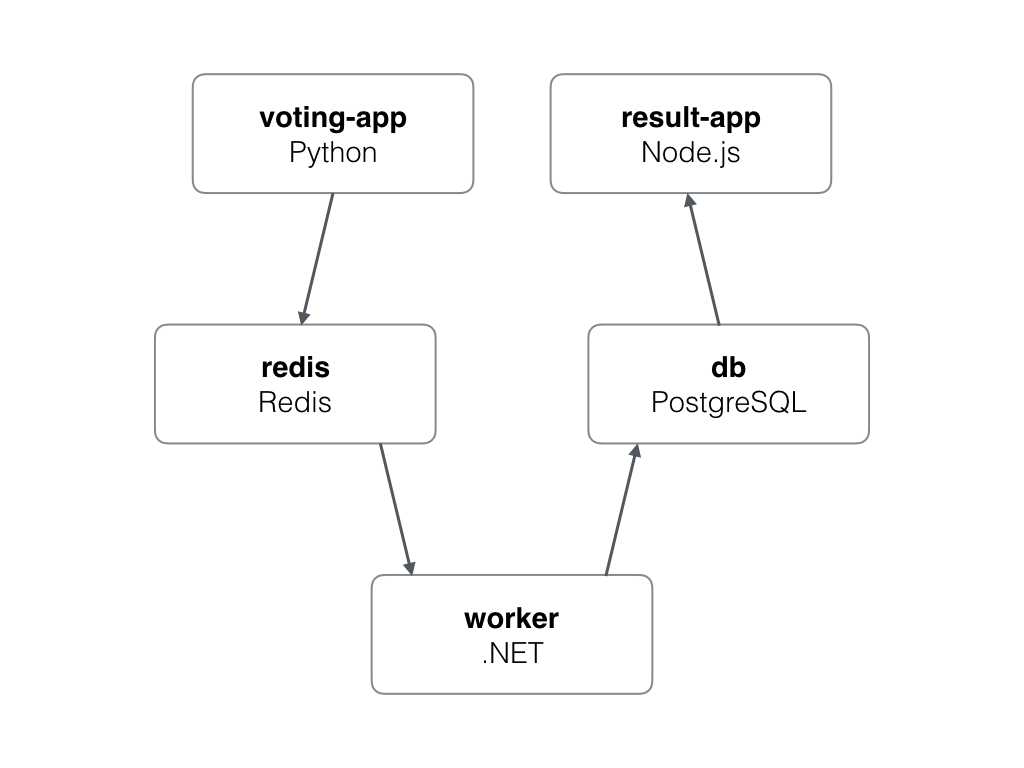
\includegraphics[width=\linewidth]{images/architecture.png}
\label{fig:votingApp}
\end{figure}

It consists of the following components:

\begin{itemize}
    \item A front-end web app
    \item A Redis database collecting new votes
    \item A worker consuming votes and storing them
    \item A Postgres database
    \item A Node.js web app showing the results\footnote{See \textit{Docker (2024)}: Example Voting App. \cite{votingGithub}}
\end{itemize}

\subsection{Application Network Map}

\subsection{LinkerD}

\subsection{Istio}

